\documentclass{article}
\usepackage[paperwidth=7.6in, paperheight=2in]{geometry}
\geometry {
    left=1mm,
    right=1mm,
}

\usepackage{tikz}
\usetikzlibrary{arrows,decorations.pathmorphing,backgrounds,positioning,fit,petri}

\begin{document}
\pagenumbering{gobble}

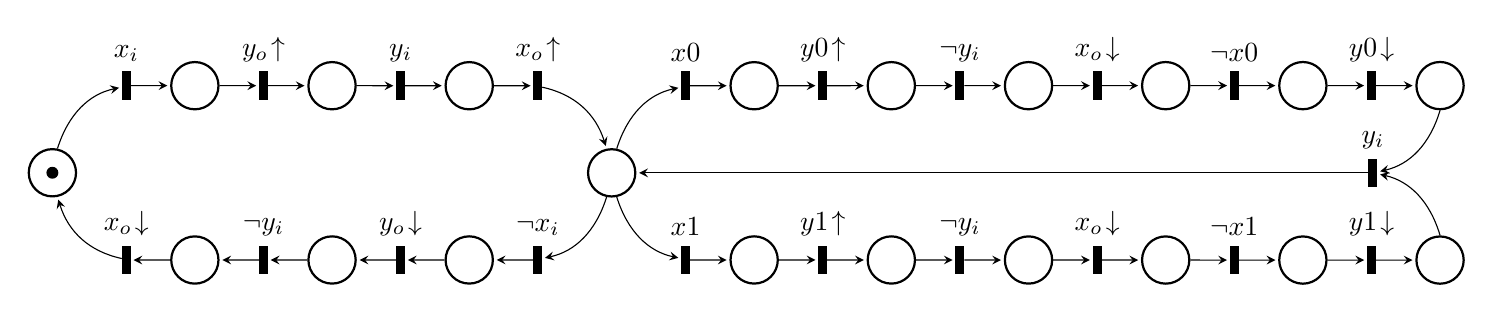
\begin{tikzpicture}[yscale=-1.1,thin,>=stealth,node distance=8mm and 5mm,
    every transition/.style={fill,minimum width=1mm,minimum height=3.5mm},
    every place/.style={draw,thick,minimum size=6mm}]

\node [place] (ready) {};

\node (l) [left=of ready] {};
\node (r0) [right=of ready] {};
\node (r1) [right=of r0, xshift=7.3cm] {};

% request branch
\node [transition] (xo+) [above=of l, label=above:$x_o\!\uparrow$] {}
    edge [post, bend right=30] (ready);
\node [place] (yi+xo+) [left=of xo+] {}
    edge [post] (xo+);

\node [transition] (yi+) [left=of yi+xo+, label=above:$y_i$] {}
    edge [post] (yi+xo+);
\node [place] (yo+yi+) [left=of yi+] {}
    edge [post] (yi+);

\node [transition] (yo+) [left=of yo+yi+, label=above:$y_o\!\uparrow$] {}
    edge [post] (yo+yi+);
\node [place] (xi+yo+) [left=of yo+] {}
    edge [post] (yo+);

\node [transition] (xi+) [left=of xi+yo+, label=above:$x_i$] {}
    edge [post] (xi+yo+);
\node (x0) [below=of xi+] {};
\node [place] (xo-xi+) [left= of x0] {}
    edge [post, bend right=30] (xi+);
\node [token] at (xo-xi+) {};

% reset branch
\node [transition] (xi-) [below=of l, label=above:$\neg x_i$] {}
    edge [pre, bend left=30] (ready);
\node [place] (xi-yo-) [left=of xi-] {}
    edge [pre] (xi-);

\node [transition] (yo-) [left=of xi-yo-, label=above:$y_o\!\downarrow$] {}
    edge [pre] (xi-yo-);
\node [place] (yo-yi-) [left=of yo-] {}
    edge [pre] (yo-);

\node [transition] (yi-) [left=of yo-yi-, label=above:$\neg y_i$] {}
    edge [pre] (yo-yi-);
\node [place] (yi-xo-) [left=of yi-] {}
    edge [pre] (yi-);

\node [transition] (xo-) [left=of yi-xo-, label=above:$x_o\!\downarrow$] {}
    edge [pre] (yi-xo-)
    edge [post, bend right=30] (xo-xi+);


% data branch

\node [transition] (x0+) [above=of r0, label=above:$x0$] {}
    edge [pre, bend left=30] (ready);
\node [place] (x0+y0+) [right=of x0+] {}
    edge [pre] (x0+);
\node [transition] (x1+) [below=of r0, label=above:$x1$] {}
    edge [pre, bend right=30] (ready);
\node [place] (x1+y1+) [right=of x1+] {}
    edge [pre] (x1+);

\node [transition] (y0+) [right=of x0+y0+, label=above:$y0\!\uparrow$] {}
    edge [pre] (x0+y0+);
\node [place] (y0+yi-) [right=of y0+] {}
    edge [pre] (y0+);
\node [transition] (y1+) [right=of x1+y1+, label=above:$y1\!\uparrow$] {}
    edge [pre] (x1+y1+);
\node [place] (y1+yi-) [right=of y1+] {}
    edge [pre] (y1+);

\node [transition] (yi-0) [right=of y0+yi-, label=above:$\neg y_i$] {}
    edge [pre] (y0+yi-);
\node [place] (yi-0xo-) [right=of yi-0] {}
    edge [pre] (yi-0);
\node [transition] (yi-1) [right=of y1+yi-, label=above:$\neg y_i$] {}
    edge [pre] (y1+yi-);
\node [place] (yi-1xo-) [right=of yi-1] {}
    edge [pre] (yi-1);

\node [transition] (xo-0) [right=of yi-0xo-, label=above:$x_o\!\downarrow$] {}
    edge [pre] (yi-0xo-);
\node [place] (xo-x0-) [right=of xo-0] {}
    edge [pre] (xo-0);
\node [transition] (xo-1) [right=of yi-1xo-, label=above:$x_o\!\downarrow$] {}
    edge [pre] (yi-1xo-);
\node [place] (xo-x1-) [right=of xo-1] {}
    edge [pre] (xo-1);

\node [transition] (x0-) [right=of xo-x0-, label=above:$\neg x0$] {}
    edge [pre] (xo-x0-);
\node [place] (x0-y0-) [right=of x0-] {}
    edge [pre] (x0-);
\node [transition] (x1-) [right=of xo-x1-, label=above:$\neg x1$] {}
    edge [pre] (xo-x1-);
\node [place] (x1-y1-) [right=of x1-] {}
    edge [pre] (x1-);

\node [transition] (y0-) [right=of x0-y0-, label=above:$y0\!\downarrow$] {}
    edge [pre] (x0-y0-);
\node [place] (y0-yi+) [right=of y0-] {}
    edge [pre] (y0-);
\node [transition] (y1-) [right=of x1-y1-, label=above:$y1\!\downarrow$] {}
    edge [pre] (x1-y1-);
\node [place] (y1-yi+) [right=of y1-] {}
    edge [pre] (y1-);

\node[transition] (yi+1) [right=of r1,label=$y_i$] {}
    edge [pre, bend left=30] (y0-yi+.south) 
    edge [pre, bend right=30] (y1-yi+.north)
    edge [post] (ready) (yi+1.west);

\end{tikzpicture}
\end{document}
